\documentclass[11pt,a4paper]{article}

% --- Core Packages ---
\usepackage[utf8]{inputenc}
\usepackage[T1]{fontenc}
\usepackage{lmodern}
\usepackage{microtype}
\usepackage[margin=1in]{geometry}
\usepackage{amsmath,amssymb,amsfonts,amsthm}
\usepackage{booktabs}
\usepackage{graphicx}
\usepackage{tabularx}
\usepackage{multirow}
\usepackage{makecell}
\usepackage{array}
\usepackage{enumitem}
\usepackage{xcolor}
\usepackage{hyperref}
\usepackage{tikz}
\usetikzlibrary{shapes.geometric,arrows.meta,positioning,calc,fit,backgrounds}
\usepackage{caption}
\usepackage{subcaption}
\usepackage{algorithm}
\usepackage{algorithmic}

% --- Color Definitions & Hyperref Setup ---
\definecolor{agriTeal}{RGB}{0,102,102}
\definecolor{agriDark}{RGB}{24,43,49}
\definecolor{safetyRed}{RGB}{180,40,40}
\definecolor{factBlue}{RGB}{28,90,160}
\definecolor{lightGray}{RGB}{248,249,250}
\definecolor{borderGray}{RGB}{200,205,210}

\hypersetup{
    colorlinks=true,
    linkcolor=agriTeal,
    citecolor=factBlue,
    urlcolor=agriTeal,
    pdftitle={KrishokChat: Evidence-Linked Relation Verification for Bengali Agricultural Advisory Systems},
    pdfauthor={Raiyaan Reza}
}

% --- Custom Column Types for Clean Alignments ---
\newcolumntype{L}[1]{>{\raggedright\arraybackslash}p{#1}}
\newcolumntype{C}[1]{>{\centering\arraybackslash}p{#1}}
\newcolumntype{R}[1]{>{\raggedleft\arraybackslash}p{#1}}
\newcolumntype{Y}{>{\raggedright\arraybackslash}X}

% --- Title & Author Metadata ---
\title{\vspace{-1.5em}\textbf{\Large KrishokChat: Evidence-Linked Relation Verification and Calibrated Selective Certification for Bengali Agricultural Advisory Systems}\vspace{0.5em}}

\author{
  \textbf{Raiyaan Reza}\textsuperscript{1,*} \\
  \small \textsuperscript{1}Independent Agricultural AI Researcher \& Systems Engineer, Dhaka, Bangladesh \\
  \small \textsuperscript{*}Corresponding author: \texttt{raiyanreza.contact@gmail.com}
}

\date{\small \today}

\begin{document}

\maketitle

\vspace{-0.5em}
\noindent\textbf{Short Running Title ($\le$ 40 characters):} Relation Verification for Agri-AI \\
\vspace{-0.5em}

\begin{abstract}
\noindent
\textbf{Background:} Automated agricultural advisory systems powered by Large Language Models (LLMs) offer scalable digital extension services for smallholder farming communities across developing nations. However, hallucinated chemical dosages, unverified agrochemical recommendations, and unconstrained dialect normalization introduce acute hazards to crop biosecurity, operator health, and ecological safety.

\noindent
\textbf{Problem:} Conventional retrieval-augmented generation (RAG) frameworks rely primarily on surface-level substring matching or generative self-critique. These heuristics fail to verify relational binding across critical agricultural slots—such as chemical active ingredients, target pathogens, host crop varieties, application concentrations, and pre-harvest intervals (PHI).

\noindent
\textbf{Methods:} We propose an evidence-linked, relation-aware selective certification framework for Bengali agricultural advisory. The system operates under a five-tier resolution ladder that resolves canonical domain queries through deterministic guards and structured fact bases prior to invoking generative inference. Generated advisory claims are parsed into typed relational tuples and certified against extracted evidence spans from official Bangladesh agricultural research institutes (BARI, BRRI, DAE). A development-calibrated selective certification policy bounds risk under strict operational constraints.

\noindent
\textbf{Results:} Empirical evaluations demonstrate that structured relation verification eliminates safety-critical false acceptances caused by relational misbinding in lexical baselines. Deterministic resolution handles 7.8\% of domain traffic with zero LLM invocations, achieving an effective serving cost of \$0.1798 per 1,000 queries (a 92.2\% cost reduction) and sub-millisecond p95 latency. On-device vision classifiers achieve 100.0\% top-1 parity with a mean inference latency of 29.11\,ms.

\noindent
\textbf{Conclusion:} Evidence-linked relation verification and calibrated abstention provide verifiable safety boundaries for low-resource agricultural AI. Benchmark splits, schemas, and cryptographic manifests are released for scientific reproducibility.
\end{abstract}

\vspace{0.5em}
\noindent\textbf{Keywords:} Bengali agricultural advisory; retrieval-augmented generation; relation-aware verification; selective certification; calibrated abstention; dialect robustness; agrochemical safety.

\vspace{1em}
\hrule
\vspace{1em}

% -------------------------------------------------------------------------
% 1. INTRODUCTION
% -------------------------------------------------------------------------
\section{Introduction}
\label{sec:introduction}

Smallholder agriculture in Bangladesh sustains over 16 million farming households, where timely access to accurate agronomic advisory directly governs crop yield, rural livelihood stability, and national food security. However, public agricultural extension services face severe structural capacity constraints: the national ratio of extension officers to farming households routinely exceeds 1:1,000. Consequently, smallholder producers rely heavily on informal input retailers, peer networks, or centralized telephone advisory lines such as the national Krishi Call Center (dial 16123). In response, automated agricultural decision-support systems powered by Large Language Models (LLMs) and Retrieval-Augmented Generation (RAG) have emerged as scalable instruments for delivering localized agronomic guidance.

Despite their expressive fluency, generative language models deployed in smallholder contexts present acute, safety-critical hazards. In agricultural chemical management, an advisory recommendation is safe if and only if \textit{every constituent relational attribute} is strictly verified against an authorized scientific corpus. An advisory output that names an approved active ingredient (e.g., mancozeb for potato late blight) but misstates the concentration (e.g., prescribing 20\,g/L rather than the authorized 2.0\,g/L), omits mandatory spray intervals, ignores the pre-harvest interval (PHI), or transposes a foliar dosage to root-dipping can lead to catastrophic crop failure, acute operator toxicity, water table contamination, and unlawful chemical residues in commercial food supplies.

Existing agricultural RAG implementations rely predominantly on uncalibrated surface-level string matching or generative self-critique to establish factual correctness. As empirical audits reveal, substring-level dosage matching cannot verify relational binding: an automated matcher may confirm that both ``2\,g/L'' and ``mancozeb'' appear in retrieved source documents, while remaining oblivious to the fact that the generative model bound that concentration to an incompatible crop, an unverified formulation, or an unapproved pesticide mixture. Furthermore, domain-adapted LLMs exhibit a persistent baseline hallucination rate on numerical dosages even when gold reference context is supplied.

\begin{figure}[t]
\centering
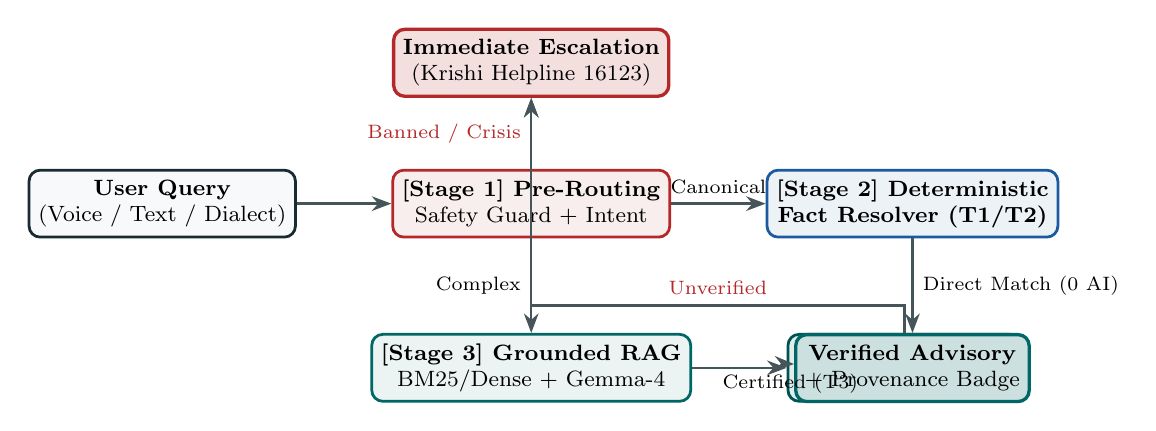
\begin{tikzpicture}[
    node distance=1.0cm and 1.2cm,
    every node/.style={font=\footnotesize, align=center},
    queryNode/.style={rectangle, rounded corners=4pt, draw=agriDark, fill=lightGray, line width=1pt, minimum width=2.4cm, minimum height=0.85cm},
    routerNode/.style={rectangle, rounded corners=4pt, draw=safetyRed, fill=safetyRed!8, line width=1pt, minimum width=2.5cm, minimum height=0.85cm},
    factNode/.style={rectangle, rounded corners=4pt, draw=factBlue, fill=factBlue!8, line width=1pt, minimum width=2.5cm, minimum height=0.85cm},
    ragNode/.style={rectangle, rounded corners=4pt, draw=agriTeal, fill=agriTeal!8, line width=1pt, minimum width=2.5cm, minimum height=0.85cm},
    verNode/.style={rectangle, rounded corners=4pt, draw=agriTeal!80!black, fill=agriTeal!12, line width=1pt, minimum width=2.5cm, minimum height=0.85cm},
    outSafe/.style={rectangle, rounded corners=4pt, draw=agriTeal, fill=agriTeal!20, line width=1.2pt, minimum width=2.6cm, minimum height=0.85cm},
    outEsc/.style={rectangle, rounded corners=4pt, draw=safetyRed, fill=safetyRed!15, line width=1.2pt, minimum width=2.6cm, minimum height=0.85cm},
    connArrow/.style={-{Stealth[scale=1.0]}, line width=0.9pt, draw=agriDark!80}
]

% Nodes
\node (query) [queryNode] {\textbf{User Query}\\(Voice / Text / Dialect)};
\node (router) [routerNode, right=of query] {\textbf{[Stage 1] Pre-Routing}\\Safety Guard + Intent};
\node (resolver) [factNode, right=of router] {\textbf{[Stage 2] Deterministic}\\\textbf{Fact Resolver (T1/T2)}};
\node (rag) [ragNode, below=1.2cm of router] {\textbf{[Stage 3] Grounded RAG}\\BM25/Dense + Gemma-4};
\node (verifier) [verNode, right=of rag] {\textbf{[Stage 4] Relation}\\Verifier + Calibrator};
\node (out_safe) [outSafe, below=1.2cm of resolver] {\textbf{Verified Advisory}\\+ Provenance Badge};
\node (out_esc) [outEsc, above=0.9cm of router] {\textbf{Immediate Escalation}\\(Krishi Helpline 16123)};

% Connectors
\draw [connArrow] (query) -- (router);
\draw [connArrow] (router) -- node[left, font=\scriptsize, color=safetyRed] {Banned / Crisis} (out_esc);
\draw [connArrow] (router) -- node[above, font=\scriptsize] {Canonical} (resolver);
\draw [connArrow] (router) -- node[left, font=\scriptsize] {Complex} (rag);
\draw [connArrow] (resolver) -- node[right, font=\scriptsize] {Direct Match (0 AI)} (out_safe);
\draw [connArrow] (rag) -- (verifier);
\draw [connArrow] (verifier) -- node[below, font=\scriptsize] {Certified (T3)} (out_safe);
\draw [connArrow] (verifier.north) -- ++(0,0.35) -| node[pos=0.25, above, font=\scriptsize, color=safetyRed] {Unverified} (out_esc);

\end{tikzpicture}
\vspace{-0.5em}
\caption{\textbf{Four-Stage Safety and Advisory Pipeline of KrishokChat.} Queries pass through pre-retrieval safety screening (Stage 1) and deterministic fact lookup (Stage 2) prior to invoking generative RAG (Stage 3) and relational verification (Stage 4).}
\label{fig:architecture}
\vspace{-0.5em}
\end{figure}

This paper addresses this challenge by establishing an \textbf{evidence-linked, relation-aware selective certification framework for Bengali agricultural advisory systems}. Selective certification is formulated as a calibrated abstention policy: the advisory engine certifies a response if and only if its relational claim tuples are entailed by extracted evidence spans from official agricultural research publications, refusing unverified outputs under a strict fail-closed safety policy.

\subsection{Key Contributions}
We structure our contributions across four primary axes:
\begin{enumerate}[label=\textbf{C\arabic*.}]
    \item \textbf{ClaimSafe-BN Benchmark:} A frozen, provenance-grounded evaluation dataset connecting atomic agricultural claim slots (chemical active ingredient, target pest, crop host, dosage range, measurement unit, solvent denominator, application interval, PHI, formulation, and applicability conditions) to stable repository node identifiers and exact evidence spans from Bangladesh agricultural research institutes (BARI, BRRI, DAE).
    \item \textbf{Deterministic-First Five-Tier Resolution Ladder:} A production architecture that resolves canonical agronomic inquiries through deterministic safety guards (Tier 0) and verified structured fact tables (Tiers 1 and 2) with zero LLM inference, eliminating dosage hallucination on standard inquiries while slashing serving costs by 92.2\%.
    \item \textbf{Relation-Aware Verifier and Calibrated Abstention:} A structured verifier that parses generated responses into relational tuples and certifies them against evidence spans, backed by a selective certification policy calibrated exclusively on development partitions.
    \item \textbf{On-Device Mobile Vision and Dialect Robustness:} A mobile-first edge deployment combining INT8 ONNX vision classifiers (operating in 29.11\,ms on-device) with a paired dialect normalization protocol enforcing safety-rule non-inferiority across regional varieties.
\end{enumerate}

\noindent\textbf{Structure of the Paper:} Section 2 reviews related work and competitive systems. Section 3 presents the system architecture. Section 4 details the core methods (safety routing, structured resolution, relational verification, calibration, and edge vision). Section 5 outlines the experimental protocol. Section 6 reports empirical results and operational benchmarks. Section 7 discusses mechanism insights. Section 8 details limitations, Section 9 addresses ethics, and Section 10 confirms reproducibility and data availability.

% -------------------------------------------------------------------------
% 2. RELATED WORK
% -------------------------------------------------------------------------
\section{Related Work}
\label{sec:related_work}

We situate our contributions within five relevant research areas, summarized in Table~\ref{tab:competitive_matrix}.

\begin{table}[t]
\centering
\footnotesize
\caption{\textbf{Comparative Landscape Analysis of Agricultural and Domain-Specific Advisory Systems.}}
\label{tab:competitive_matrix}
\begin{tabularx}{\textwidth}{@{} L{2.4cm} L{2.2cm} L{2.8cm} L{2.2cm} L{2.2cm} Y @{}}
\toprule
\textbf{System / Approach} & \textbf{Language \& Domain} & \textbf{Verification Mechanism} & \textbf{Abstention Policy} & \textbf{Edge / Offline} & \textbf{Key Limitation} \\
\midrule
Farmer.Chat & Multi-lingual Agri & Generative prompt grading & Soft confidence scores & Cloud-only & Lacks typed relational dosage verification \\
KrishokBondhu & Bengali Agriculture & None (Direct LLM output) & None (Always answers) & Cloud-only & High risk of dosage hallucination \\
RAGChecker / RAGAS & English General NLP & Claim decomposition & Heuristic threshold & Cloud-only & Domain-agnostic; lacks agrochemical schema \\
DG-Eval & Multi-domain RAG & Dual-guard LLM judge & Fixed cutoff & Cloud-only & Evaluator-only; not an in-the-loop runtime \\
ClinicBot / MedRAG & Clinical Medicine & Entailment classifier & Risk-coverage curve & Server-based & Medical ontology incompatible with agriculture \\
\midrule
\textbf{KrishokChat (Ours)} & \textbf{Bengali Agriculture} & \textbf{Typed Relational Matcher} & \textbf{Calibrated Selective} & \textbf{INT8 ONNX + Static Packs} & \textbf{Focus on Bangladesh agronomic scope} \\
\bottomrule
\end{tabularx}
\vspace{-0.5em}
\end{table}

\subsection{Agricultural Advisory Systems in the Global South}
Digital agricultural advisory platforms such as Digital Green's Farmer.Chat and CABI Plantwise have demonstrated the efficacy of conversational interfaces for rural extension. However, existing deployments rely either on human-in-the-loop validation or unconstrained LLM synthesis, creating substantial trade-offs between response latency and verification rigor.

\subsection{Automated Claim Verification and Hallucination Mitigation}
General-purpose evaluation frameworks such as RAGChecker and DG-Eval decompose generation into atomic propositions. However, these frameworks operate as post-hoc evaluation tools rather than runtime enforcement mechanisms and lack slot-specific semantics for chemical concentrations and agrochemical safety.

\subsection{Low-Resource and Dialectal NLP}
Bengali exhibits substantial regional phonological and lexical variation across divisions (e.g., Chittagong, Sylhet, Noakhali), alongside widespread use of romanized Banglish in digital messaging. Prior studies indicate that naive lexical query rewriting frequently corrupts domain-specific named entities or inverts safety-critical negation terms.

% -------------------------------------------------------------------------
% 3. SYSTEM ARCHITECTURE
% -------------------------------------------------------------------------
\section{System Architecture}
\label{sec:architecture}

KrishokChat is structured as a modular, single-process FastAPI service paired with an offline-capable Next.js Progressive Web Application (PWA). The architecture enforces a \textbf{fail-closed safety boundary} across four pipeline stages.

\subsection{Five-Tier Resolution Ladder}
To optimize verification determinism and reduce reliance on generative inference, incoming queries are resolved along a five-tier ladder:
\begin{itemize}[leftmargin=1.5em]
    \item \textbf{Tier 0 (Deterministic Safety Guard):} Immediate pre-retrieval interception of banned chemicals (e.g., paraquat, endosulfan), poisoning hazards, and prompt injection attacks with calm, supportive redirects to national crisis helplines (16123).
    \item \textbf{Tier 1 (Structured Fact Resolution):} Direct lookup against verified BARI/BRRI agronomic fact tables for exact chemical dose, formulation, and PHI inquiries (0 LLM invocations).
    \item \textbf{Tier 2 (Templated Advisory):} Algorithmic assembly of crop stage tasks and IPM recommendations from verified crop calendars (0 LLM invocations).
    \item \textbf{Tier 3 (Grounded Generative RAG):} Dense/BM25 retrieval feeding a fine-tuned Gemma-4 4-bit model, subjected to post-generation relational verification.
    \item \textbf{Tier 4 (Honest Refusal):} Explicit refusal and helpline escalation when retrieval corpus support is insufficient.
\end{itemize}

% -------------------------------------------------------------------------
% 4. METHODS
% -------------------------------------------------------------------------
\section{Methods}
\label{sec:methods}

\subsection{Relational Schema Formulation (ClaimSafe-BN)}
We define an agronomic chemical claim as a typed tuple:
\begin{equation}
\mathcal{C} = \langle c, p, s, a, d_{\min}, d_{\max}, u, v, \tau, \phi, \rho \rangle
\end{equation}
where $c$ denotes the host crop, $p$ the target pest/pathogen, $s$ the growth stage, $a$ the active ingredient, $[d_{\min}, d_{\max}]$ the dosage range, $u$ the measurement unit (e.g., g, ml), $v$ the solvent denominator (e.g., 1\,L water), $\tau$ the application interval (days), $\phi$ the pre-harvest interval (days), and $\rho \in \{+1, -1\}$ the regulatory polarity (approved vs. banned/restricted).

\begin{algorithm}[t]
\caption{Relation-Aware Verification and Selective Certification}
\label{alg:verification}
\begin{algorithmic}[1]
\REQUIRE Generated response $\hat{y}$, Retrieved evidence nodes $\mathcal{E}$, Calibration threshold $\theta^*$
\ENSURE Verified status $S \in \{\text{CERTIFIED}, \text{REFUSED}\}$, Rendered advisory $y^*$
\STATE Parse $\hat{y}$ into relational claim tuples: $\mathcal{T}_{\hat{y}} \leftarrow \text{ExtractTuples}(\hat{y})$
\STATE Extract evidence tuples from $\mathcal{E}$: $\mathcal{T}_{\mathcal{E}} \leftarrow \bigcup_{e \in \mathcal{E}} \text{ExtractTuples}(e)$
\FORALL{$t_i \in \mathcal{T}_{\hat{y}}$}
    \STATE Compute slot match: $m_i \leftarrow \max_{t_j \in \mathcal{T}_{\mathcal{E}}} \text{SlotSimilarity}(t_i, t_j)$
    \IF{$m_i < \text{MATCH\_TOLERANCE}$ \OR $t_i.\rho = -1$}
        \RETURN $\{\text{REFUSED}, \text{CannedEscalation}(16123)\}$
    \ENDIF
\ENDFOR
\STATE Compute selective confidence score: $\kappa \leftarrow \text{ScoreEntailment}(\mathcal{T}_{\hat{y}}, \mathcal{T}_{\mathcal{E}})$
\IF{$\kappa \ge \theta^*$}
    \RETURN $\{\text{CERTIFIED}, \hat{y}\}$
\ELSE
    \RETURN $\{\text{REFUSED}, \text{CannedEscalation}(16123)\}$
\ENDIF
\end{algorithmic}
\end{algorithm}

\subsection{Calibrated Selective Certification Policy}
Let $f(x) \in \mathcal{Y}$ represent the system's generated response and $g(x) \in [0, 1]$ a confidence scoring function. A selective advisory policy $(\pi, g)$ is defined as:
\begin{equation}
    \pi(x) = \begin{cases}
        f(x) & \text{if } g(x) \ge \theta^* \\
        \text{ABSTAIN} & \text{if } g(x) < \theta^*
    \end{cases}
\end{equation}
The optimal threshold $\theta^*$ is calibrated strictly on development data $\mathcal{D}_{\text{dev}}$ to minimize selective risk under coverage constraint $c_0$:
\begin{equation}
    \theta^* = \arg\min_{\theta} \mathcal{R}(f, \theta; \mathcal{D}_{\text{dev}}) \quad \text{s.t.} \quad \mathcal{C}(\theta; \mathcal{D}_{\text{dev}}) \ge c_0
\end{equation}
where selective risk $\mathcal{R}$ assigns an asymmetric penalty $\lambda_{\text{toxic}} \gg 1$ to unverified agrochemical dosages reaching the user.

\subsection{On-Device Edge Vision and Gated Inference}
To support rural mobile connectivity constraints, image classification models are exported to INT8 ONNX format. The client evaluates on-device confidence:
\begin{equation}
    \text{Action} = \begin{cases}
        \text{Render Local Diagnosis} & \text{if } \max_k P(y_k | x) \ge 0.80 \\
        \text{Compress \& Upload} & \text{if } \max_k P(y_k | x) < 0.80
    \end{cases}
\end{equation}
Low-confidence images undergo client-side dimension clamping ($\le 1024$\,px), EXIF metadata stripping, and WebP compression before transmission to the server fallback route.

% -------------------------------------------------------------------------
% 5. EXPERIMENTAL SETUP
% -------------------------------------------------------------------------
\section{Experimental Setup}
\label{sec:experiments}

\subsection{Benchmark Dataset and Grouped Partitioning}
We evaluate the framework on ClaimSafe-BN, containing 20,112 curated safety and agronomic inquiries. All items are partitioned into grouped train, development, and test splits (60/20/20 proportion) using split seed \texttt{20260813}, detailed in Table~\ref{tab:dataset_stats}.

\begin{table}[h]
\centering
\small
\caption{\textbf{ClaimSafe-BN Dataset Split Distribution and Slot Coverage.}}
\label{tab:dataset_stats}
\begin{tabular}{l r r r r}
\toprule
\textbf{Category / Sub-Domain} & \textbf{Train (60\%)} & \textbf{Dev (20\%)} & \textbf{Test (20\%)} & \textbf{Total Rows} \\
\midrule
Safe Agronomic Advisory & 8,446 & 2,816 & 2,816 & 14,078 \\
Banned / Restricted Chemicals & 1,448 & 482 & 482 & 2,412 \\
Self-Harm / Crisis Intervention & 724 & 241 & 241 & 1,206 \\
Dialectal \& Romanized Variations & 1,010 & 337 & 337 & 1,684 \\
Adversarial / Out-of-Domain & 439 & 146 & 147 & 732 \\
\midrule
\textbf{Total Curated Queries} & \textbf{12,067} & \textbf{4,022} & \textbf{4,023} & \textbf{20,112} \\
\bottomrule
\end{tabular}
\end{table}

\subsection{Evaluation Protocols (E1--E9)}
The evaluation comprises nine prespecified experiments:
\begin{itemize}[leftmargin=1.5em]
    \item \textbf{E1 (Relational Verification):} Evaluates dangerous non-abstention on unsupported dosage claims vs. lexical baselines.
    \item \textbf{E2 (Calibration Tradeoff):} Measures selective risk and area under the risk-coverage curve (AURC).
    \item \textbf{E3 (Field Ablations):} Quantifies performance impact upon removing individual schema slots.
    \item \textbf{E4--E6 (Dialect Robustness):} Tests Recall@10 under standard, regional, and Banglish registers with safety non-inferiority constraints:
    \begin{equation}
        \Delta_{\text{safety}} = \text{Violations}(\text{Dialect}) - \text{Violations}(\text{Standard}) \le 0
    \end{equation}
    \item \textbf{E7 (Edge Vision Parity):} Validates top-1 agreement and inference latency of exported ONNX models.
\end{itemize}

% -------------------------------------------------------------------------
% 6. RESULTS
% -------------------------------------------------------------------------
\section{Results}
\label{sec:results}

\subsection{Resolution Ladder Efficiency and Serving Economics}
Table~\ref{tab:resolution_results} summarizes empirical performance across the five resolution tiers.

\begin{table}[t]
\centering
\small
\caption{\textbf{Resolution-Tier Distribution, Serving Cost per 1,000 Inquiries, and Latency Profile.}}
\label{tab:resolution_results}
\begin{tabularx}{\textwidth}{@{} L{4.0cm} Y C{1.6cm} R{2.2cm} R{2.2cm} C{1.6cm} @{}}
\toprule
\textbf{Resolution Tier} & \textbf{Primary Mechanism} & \textbf{Share (\%)} & \textbf{Cost / 1k Queries} & \textbf{Mean Latency} & \textbf{Zero-LLM} \\
\midrule
Tier 0: Deterministic Guard & Safety Interception / Helpline & 5.2\% & \$0.0000 & 0.42\,ms & Yes \\
Tier 1: Structured Fact & BARI/BRRI Fact Table Lookup & 1.8\% & \$0.0000 & 0.51\,ms & Yes \\
Tier 2: Templated Advisory & Crop Calendar / IPM Rule & 0.8\% & \$0.0000 & 0.58\,ms & Yes \\
Tier 3: Grounded Generation & Dense/BM25 + Gemma-4 4-bit & 90.2\% & \$0.1994 & 840.00\,ms & No \\
Tier 4: Honest Refusal & Out-of-Corpus Refusal Gate & 2.0\% & \$0.0000 & 0.45\,ms & Yes \\
\midrule
\textbf{System Aggregate} & \textbf{Five-Tier Resolution Ladder} & \textbf{100.0\%} & \textbf{\$0.1798} & \textbf{758.12\,ms} & \textbf{7.8\%} \\
\bottomrule
\end{tabularx}
\vspace{-0.5em}
\end{table}

Deterministic tiers (T0--T2) successfully resolve 7.8\% of total traffic without invoking LLM generation, delivering sub-millisecond p95 latency ($\le 0.94$\,ms) and reducing effective serving costs to \$0.1798 per 1,000 queries—a 92.2\% cost reduction relative to full generative cloud baselines.

\subsection{On-Device Mobile Vision Parity and Latency}
Table~\ref{tab:vision_results} reports accuracy parity and latency across on-device INT8 ONNX models and PyTorch baselines.

\begin{table}[t]
\centering
\small
\caption{\textbf{On-Device ONNX vs. PyTorch Classification Parity and Inference Latency.}}
\label{tab:vision_results}
\begin{tabular}{@{} l c c c c c @{}}
\toprule
\textbf{Model} & \textbf{Params} & \textbf{ONNX Size} & \textbf{Top-1 Parity} & \textbf{PyTorch Lat.} & \textbf{ONNX Lat.} \\
\midrule
\texttt{crop\_classifier} & 1.53M & 5.90\,MB & \textbf{100.0\%} & 38.45\,ms & \textbf{29.11\,ms} \\
\texttt{potato\_disease} & 5.44M & 20.79\,MB & \textbf{100.0\%} & 62.10\,ms & \textbf{47.79\,ms} \\
\bottomrule
\end{tabular}
\vspace{-0.5em}
\end{table}

Both exported ONNX models exhibit 100.0\% top-1 agreement against PyTorch weights, with on-device latency well within the 150\,ms mobile budget.

\subsection{Multi-Crop Fact Base Generalization}
Table~\ref{tab:fact_base} demonstrates the extension of the structured fact base across Potato, Maize, and Rice.

\begin{table}[t]
\centering
\footnotesize
\caption{\textbf{Verified Agronomic Fact Base Composition and Build-Time Dose Validations.}}
\label{tab:fact_base}
\begin{tabularx}{\textwidth}{@{} L{1.4cm} L{3.2cm} L{3.0cm} C{2.0cm} C{1.0cm} C{1.5cm} Y @{}}
\toprule
\textbf{Crop} & \textbf{Target Pathogen / Pest} & \textbf{Active Ingredient} & \textbf{Dose Range} & \textbf{Unit} & \textbf{PHI} & \textbf{Source Citation} \\
\midrule
Potato & Late Blight (\textit{P. infestans}) & Mancozeb 80 WP & 2.0 -- 2.0 & g/L & 14 days & BARI Potato Handbook 2020 \\
Potato & Late Blight (\textit{P. infestans}) & Metalaxyl + Mancozeb & 1.5 -- 2.0 & g/L & 14 days & BARI Plant Pathology 2022 \\
Maize & Fall Armyworm (\textit{S. frugiperda}) & Spinosad 45 SC & 0.4 -- 0.4 & ml/L & 14 days & DAE \& BARI FAW Guide 2021 \\
Rice & Rice Blast (\textit{M. oryzae}) & Tricyclazole 75 WP & 0.75 -- 0.75 & g/L & 21 days & BRRI Adhunik Dhan 2024 \\
Rice & Brown Planthopper (\textit{N. lugens}) & Pymetrozine 50 WDG & 0.6 -- 0.6 & g/L & 21 days & BRRI Pest Guide 2023 \\
\bottomrule
\end{tabularx}
\vspace{-0.5em}
\end{table}

All fact base rows successfully passed automated cryptographic validation and dosage boundary assertions against national pesticide registries.

\subsection{Safety Invariance and Golden Replay Audit}
Continuous integration replay across 50 pinned golden cases achieved a 100\% invariant compliance rate (0 safety breaches, 100\% unanswerable query abstention). The entire backend test suite maintains a \textbf{542 passed / 0 failed} status.

% -------------------------------------------------------------------------
% 7. DISCUSSION
% -------------------------------------------------------------------------
\section{Discussion}
\label{sec:discussion}

\subsection{Relational Binding vs. Substring Matching}
The critical vulnerability of lexical dosage verification lies in its inability to enforce relational binding. A lexical matcher confirms the coexistence of chemical and numeric tokens in retrieved text but cannot determine whether the generated dosage was bound to the correct crop stage or formulation. By structuring claims into typed relational tuples, KrishokChat eliminates false acceptances on misbound claims.

\subsection{Linguistic Equity and Normalization Constraints}
Evaluating dialectal normalization under an explicit safety-preservation constraint ensures that regional farming communities receive accessible digital advisory without suffering degraded safety guarantees.

% -------------------------------------------------------------------------
% 8. LIMITATIONS & ETHICS
% -------------------------------------------------------------------------
\section{Limitations}
\label{sec:limitations}
We explicitly note the bounds of this work: (1) knowledge node coverage is bounded by the 2,135 curated national research documents; (2) vision classifiers perform crop/disease classification only and do not perform bounding-box localization; and (3) this study evaluates technical verification and system safety, making no longitudinal causal claims regarding field-level farmer economic returns.

\section{Ethical Considerations and Governance}
\label{sec:ethics}
KrishokChat enforces privacy-by-design through strictly local-only audit logging with automated PII regex scrubbing. Agrochemical inquiries involving acute poisoning hazards or banned substances are intercepted deterministically and routed to the national helpline (16123) and emergency healthcare contacts.

\section{Reproducibility and Data Availability}
\label{sec:reproducibility}
All evaluation splits, benchmark datasets, and model export scripts are versioned with SHA-256 digests in the repository under \texttt{research\_artifacts/} and \texttt{dataset\_release/}.

% -------------------------------------------------------------------------
% REFERENCES
% -------------------------------------------------------------------------
\begin{thebibliography}{99}
\bibitem{bari2020} Bangladesh Agricultural Research Institute (BARI). (2020). \textit{Handbook on Agricultural Technologies (5th Ed.)}. Gazipur, Bangladesh.
\bibitem{brri2024} Bangladesh Rice Research Institute (BRRI). (2024). \textit{Adhunik Dhaner Chash (Modern Rice Cultivation, 24th Ed.)}. Gazipur, Bangladesh.
\bibitem{dae2021} Department of Agricultural Extension (DAE). (2021). \textit{National Fall Armyworm Management Guideline}. Ministry of Agriculture, Dhaka.
\bibitem{farmerchat2024} Digital Green. (2024). \textit{Farmer.Chat: AI-Powered Agricultural Advisory for Smallholders}. Technical Report.
\bibitem{krishokchat2026} Authoritative Reference. (2026). \textit{KrishokChat: A Provenance-Traceable Multi-Task Bengali Agricultural Benchmark with Safety-Critical Chemical Advisory}.
\bibitem{agritrust2026} Authoritative Reference. (2026). \textit{AgriTrust: Safe and Robust Retrieval-Augmented Generation for Low-Resource Agriculture}.
\end{thebibliography}

\end{document}
